\documentclass[10pt,a4paper,twoside]{article}\usepackage[]{graphicx}\usepackage[]{xcolor}
% maxwidth is the original width if it is less than linewidth
% otherwise use linewidth (to make sure the graphics do not exceed the margin)
\makeatletter
\def\maxwidth{ %
  \ifdim\Gin@nat@width>\linewidth
    \linewidth
  \else
    \Gin@nat@width
  \fi
}
\makeatother

\definecolor{fgcolor}{rgb}{0.345, 0.345, 0.345}
\newcommand{\hlnum}[1]{\textcolor[rgb]{0.686,0.059,0.569}{#1}}%
\newcommand{\hlsng}[1]{\textcolor[rgb]{0.192,0.494,0.8}{#1}}%
\newcommand{\hlcom}[1]{\textcolor[rgb]{0.678,0.584,0.686}{\textit{#1}}}%
\newcommand{\hlopt}[1]{\textcolor[rgb]{0,0,0}{#1}}%
\newcommand{\hldef}[1]{\textcolor[rgb]{0.345,0.345,0.345}{#1}}%
\newcommand{\hlkwa}[1]{\textcolor[rgb]{0.161,0.373,0.58}{\textbf{#1}}}%
\newcommand{\hlkwb}[1]{\textcolor[rgb]{0.69,0.353,0.396}{#1}}%
\newcommand{\hlkwc}[1]{\textcolor[rgb]{0.333,0.667,0.333}{#1}}%
\newcommand{\hlkwd}[1]{\textcolor[rgb]{0.737,0.353,0.396}{\textbf{#1}}}%
\let\hlipl\hlkwb

\usepackage{framed}
\makeatletter
\newenvironment{kframe}{%
 \def\at@end@of@kframe{}%
 \ifinner\ifhmode%
  \def\at@end@of@kframe{\end{minipage}}%
  \begin{minipage}{\columnwidth}%
 \fi\fi%
 \def\FrameCommand##1{\hskip\@totalleftmargin \hskip-\fboxsep
 \colorbox{shadecolor}{##1}\hskip-\fboxsep
     % There is no \\@totalrightmargin, so:
     \hskip-\linewidth \hskip-\@totalleftmargin \hskip\columnwidth}%
 \MakeFramed {\advance\hsize-\width
   \@totalleftmargin\z@ \linewidth\hsize
   \@setminipage}}%
 {\par\unskip\endMakeFramed%
 \at@end@of@kframe}
\makeatother

\definecolor{shadecolor}{rgb}{.97, .97, .97}
\definecolor{messagecolor}{rgb}{0, 0, 0}
\definecolor{warningcolor}{rgb}{1, 0, 1}
\definecolor{errorcolor}{rgb}{1, 0, 0}
\newenvironment{knitrout}{}{} % an empty environment to be redefined in TeX

\usepackage{alltt}

%%% Load some LaTeX packages:
\usepackage{amsmath}                       % for mathematical features 
\usepackage[left=2.5cm,top=3cm,bottom=3cm,right=2.5cm]{geometry}   % text margins
\usepackage{booktabs}                      % for booktabs in print(xtable)).
\usepackage{authblk}                       % for footnote style author/affiliation
\usepackage{amssymb}
\usepackage{amsthm}
% LaTeX package for captions customization:
\usepackage[margin=10pt,font=small,labelfont=bf,format=hang]{caption}
\usepackage{hyperref}                      % Hyperlinks and \url{}
\hypersetup{
    colorlinks=true, % Enable colored text for links instead of drawing boxes
    linkcolor=blue,  % Color for internal document links (e.g., sections, equations, figures, tables)
    citecolor=blue,  % Color for bibliographic citation links (e.g., \cite{})
    urlcolor=blue    % Color for external web URLs (e.g., \url{})
}

% Import the natbib package and sets a bibliography  and citation styles
% https://www.overleaf.com/learn/latex/Natbib_citation_styles
\usepackage[super,square,comma,sort&compress,numbers]{natbib}
\bibliographystyle{unsrtnat}
\usepackage[nottoc]{tocbibind} % For bibliography in the table of contents but no "Chapter" or "Section" label inside


%%%%%%%%%%%%
%%%%
%%%% BEGIN scientific and R commands
%%%%
%%%%%%%%%%%%

% Operadores y Funciones
\DeclareMathOperator{\var}{var}             % variance
\DeclareMathOperator{\logit}{logit}         % logit function
\newcommand{\logodds}{\text{logodds}}       % logodds
\newcommand{\E}{\mathbb{E}}                 % expectation
\newcommand{\equaldef}{\stackrel{\text{def}}{=}}  % equal by definition


% Distribuciones de probabilidad
\DeclareMathOperator{\Bern}{Bern}           % Bernoulli
\DeclareMathOperator{\Bin}{Bin}             % Binomial
\DeclareMathOperator{\Pois}{Pois}           % Poisson
\DeclareMathOperator{\LogN}{LogN}           % lognormal
\DeclareMathOperator{\NB}{NB}               % Negative Binimial
\newcommand{\Normal}{\mathcal{N}}           % normal (distribution)


%%% Epidemiologic notation:
% text version (within equation):
\newcommand{\CI}{\text{CI}}                 % cumulative incidence
\newcommand{\RD}{\text{RD}}                 % risk difference
\newcommand{\RR}{\text{RR}}                 % risk ratio
\newcommand{\OR}{\text{OR}}                 % odds ratio
\newcommand{\PR}{\text{PR}}                 % prevalence ratio
\newcommand{\PD}{\text{PD}}                 % prevalence difference
\newcommand{\IRR}{\text{IRR}}               % incidence rate ratio
\newcommand{\IRD}{\text{IRD}}               % incidence rate difference
\newcommand{\odds}{\text{odds}}             % odds
\newcommand{\PAR}{\text{PAR}}               % population attributable risk
\newcommand{\EAR}{\text{EAR}}               % exposure attributable risk
\newcommand{\MR}{\text{MR}}                 % mortality rate
\newcommand{\MRR}{\text{MRR}}               % mortality rate ratio
\newcommand{\DSMR}{\text{MR}_{\text{DS}}}   % directly standardized mortality rate
\newcommand{\ISMR}{\text{MR}_{\text{IS}}}   % indirectly standardized mortality rate
\newcommand{\CMF}{\text{CMF}}               % Comparative mortality figure
\newcommand{\SMR}{\text{SMR}}               % Standardized mortality ratio
\newcommand{\AMR}{\text{AMR}}               % Adjusted Mortality Rate 


%%% R notation:
\newcommand{\Robject}[1]{\texttt{#1}}
\newcommand{\Rpackage}[1]{\textsf{#1}}
\newcommand{\Rclass}[1]{\textit{#1}}
\newcommand{\R}{\textsf{R}}
\newcommand{\Rfun}[1]{\texttt{#1\hspace{-0.15em}()}}
\newcommand{\Rmethod}[1]{\texttt{#1}}
\newcommand{\Rarg}[1]{\texttt{#1}}
\newcommand{\Rcode}[1]{\texttt{#1}}

%%%%%%%%%%%%
%%%%
%%%% END scientific and R commands
%%%%
%%%%%%%%%%%%









\IfFileExists{upquote.sty}{\usepackage{upquote}}{}
\begin{document}

% Activate lowercase Roman numerals for the preliminary pages
\pagenumbering{roman}


% Title page
\title{Integrating \R\ and \LaTeX\ in a single source document with the \Rpackage{knitr} package: An example of reporting reproducible research\vspace{1mm} \normalsize{\color{blue}(version 4.4)}}
\author[1,2]{Jose Barrera}
\affil[1]{\small ISGlobal Barcelona Institute for Global Health - Campus Mar}
\affil[2]{\small Departament de Matem\`atiques, Universitat Aut\`onoma de Barcelona}

\maketitle
\thispagestyle{empty} % (page i internally but hidden)


% Pagina 2 (ii): Blank page after the title pager
\clearpage
\thispagestyle{empty}
\null
\clearpage


%%%%%%%%%%%%%%%
%%%
%%% Abstract page -> Page 3 (iii)
%%%
%%%%%%%%%%%%%%%
\begin{abstract}
Here you can put your abstract...
\end{abstract}


% Pagina 4 (iv): Blank page after the abstract
\clearpage
\thispagestyle{empty}
\null
\clearpage



%%%%%%%%%%%%%%%
%%%
%%% Table of contents -> Page 5 (v)
%%%
%%%%%%%%%%%%%%%
\tableofcontents


% Pagina 6 (vi): Blank page after the table of contents
% Leave or remove this page blank so that the first page
% of the first section is located on an odd-numbered page
% in the PDF resulting from compiling the Rnw
\clearpage
\thispagestyle{empty}
\null
\clearpage


% Change to Arabic numeral numbering (starts at 1) for Section 1
\pagenumbering{arabic}


%%%%%%%%%%%%%%%
%%%
%%% Section: Introduction
%%%
%%%%%%%%%%%%%%%
\section{Introduction}
\label{sec:intro}
This report is an example of reproducible research using the function \Rfun{knit}, in the \R\ package \Rpackage{knitr}, and \LaTeX. For an introduction to \Rpackage{knitr}, I recommend the website of the package\cite{knitr}.

%%%%%%%%%%%%%%%
%%%
%%% Subsection: 
%%%
%%%%%%%%%%%%%%%
\subsection{Toy example}
\label{sec:toy}
The aim of this document is to provide a minimal example of a \Robject{Rnw} source file that integrates code of both \R\ and \LaTeX, which result is this PDF file. The statistical analysis shown in this document, a linear regression fitting, is only for illustration purposes on how \Robject{knitr} works  and should not be considered for statistical purposes. In Section \ref{sec:data} we explore data graphically. Then, in Section \ref{sec:modeling}, we fit and interpret a linear regression model. The \R\ code used is shown in Appendix \ref{app:Rcode}. Appendix \ref{app:libraries} shows the \R\ packages we need to get the PDF for this document.

%%%%%%%%%%%%%%%
%%%
%%% Section: Data
%%%
%%%%%%%%%%%%%%%
\section{Data}
\label{sec:data}
Figure \ref{fig:dataplot}\footnote{See Appendix \ref{app:data}.} shows a graphical representation of the relationship between the wind speed and ozone levels, where we can see a possible linear association:

\begin{equation}
\label{eq:model}
\text{Ozone} = \beta_0 + \beta_1 \text{Wind speed}
\end{equation}


\begin{knitrout}\footnotesize
\definecolor{shadecolor}{rgb}{0.969, 0.969, 0.969}\color{fgcolor}\begin{figure}[ht]

{\centering 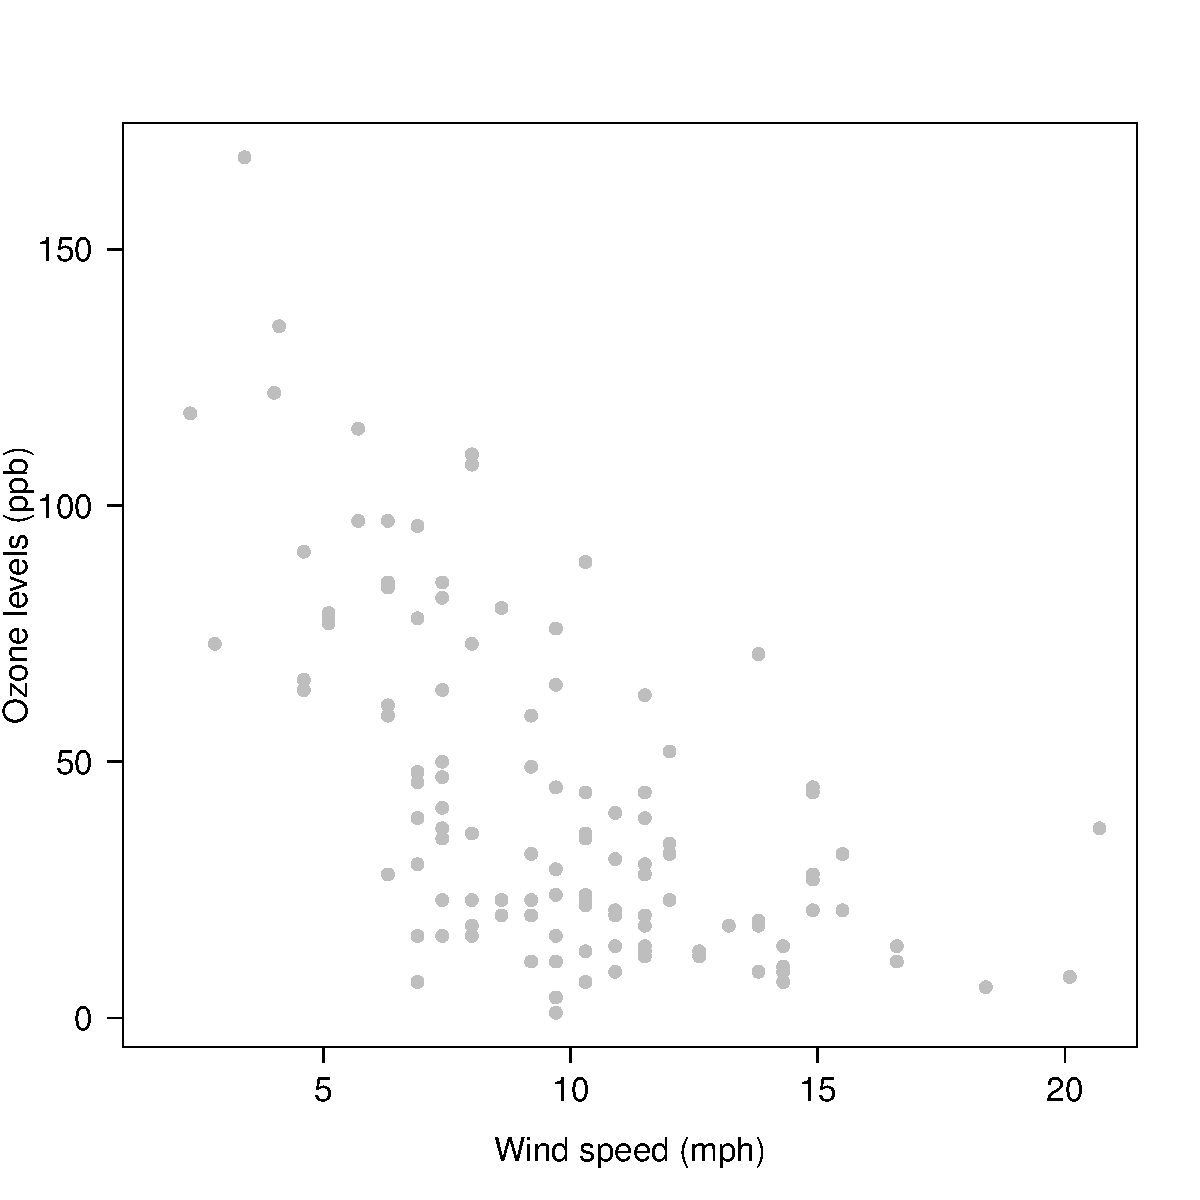
\includegraphics[width=0.45\textwidth]{figure/dataplot-1} 

}

\caption{\label{fig:dataplot}Scatter plot of ozone levels vs. wind speed.}\label{fig:dataplot}
\end{figure}

\end{knitrout}



%%%%%%%%%%%%%%%
%%%
%%% Section: Modeling
%%%
%%%%%%%%%%%%%%%
\section{Modeling}
\label{sec:modeling}


\begin{knitrout}\footnotesize
\definecolor{shadecolor}{rgb}{0.969, 0.969, 0.969}\color{fgcolor}\begin{kframe}
\begin{verbatim}
##              Estimate Std. Error  t value     Pr(>|t|)
## (Intercept) 96.872895  7.2386887 13.38266 3.992068e-25
## Wind        -5.550923  0.6904021 -8.04013 9.271974e-13
\end{verbatim}
\end{kframe}
\end{knitrout}




In Section \ref{sec:data} we have seen that a there is a possible linear relationship between the wind speed and the ozone levels, under model \eqref{eq:model}. Thus, we can try to fit a linear regression model\footnote{See \R\ code in Appendix \ref{app:model}.}. Specifically, Table \ref{tab:coeftable} shows the estimated coefficients of the linear model\footnote{The vignette ``The \Rpackage{xtable}\ Gallery''\cite{xtablegallery} provides a lot of examples for table customization.}. Under this model, a one unit increase in the wind speed is associated to a decrease of 5.55 units in the mean of ozone levels. Figure \ref{fig:modelplot} shows the data as well as the fitted model.

% latex table generated in R 4.5.0 by xtable 1.8-8 package
% Sat Oct 24 13:22:15 2026
\begin{table}[ht]
\centering
\begingroup\footnotesize
\begin{tabular}{rrrrr}
  \toprule
 & \multicolumn{1}{c}{\bf Estimate} & \multicolumn{1}{c}{\bf Std.~Error} & \multicolumn{1}{c}{\(\boldsymbol{t}\)\bf{-value}} & \multicolumn{1}{c}{\(\boldsymbol{p}\)\bf{-value}} \\ 
  \midrule
(Intercept) & 96.87 & 7.24 & 13.38 & 0.0000 \\ 
  Wind & -5.55 & 0.69 & -8.04 & 0.0000 \\ 
   \bottomrule
\end{tabular}
\endgroup
\caption{Linear regression model coefficients for wind and ozone association.} 
\label{tab:coeftable}
\end{table}



\begin{knitrout}\footnotesize
\definecolor{shadecolor}{rgb}{0.969, 0.969, 0.969}\color{fgcolor}\begin{figure}[ht]

{\centering 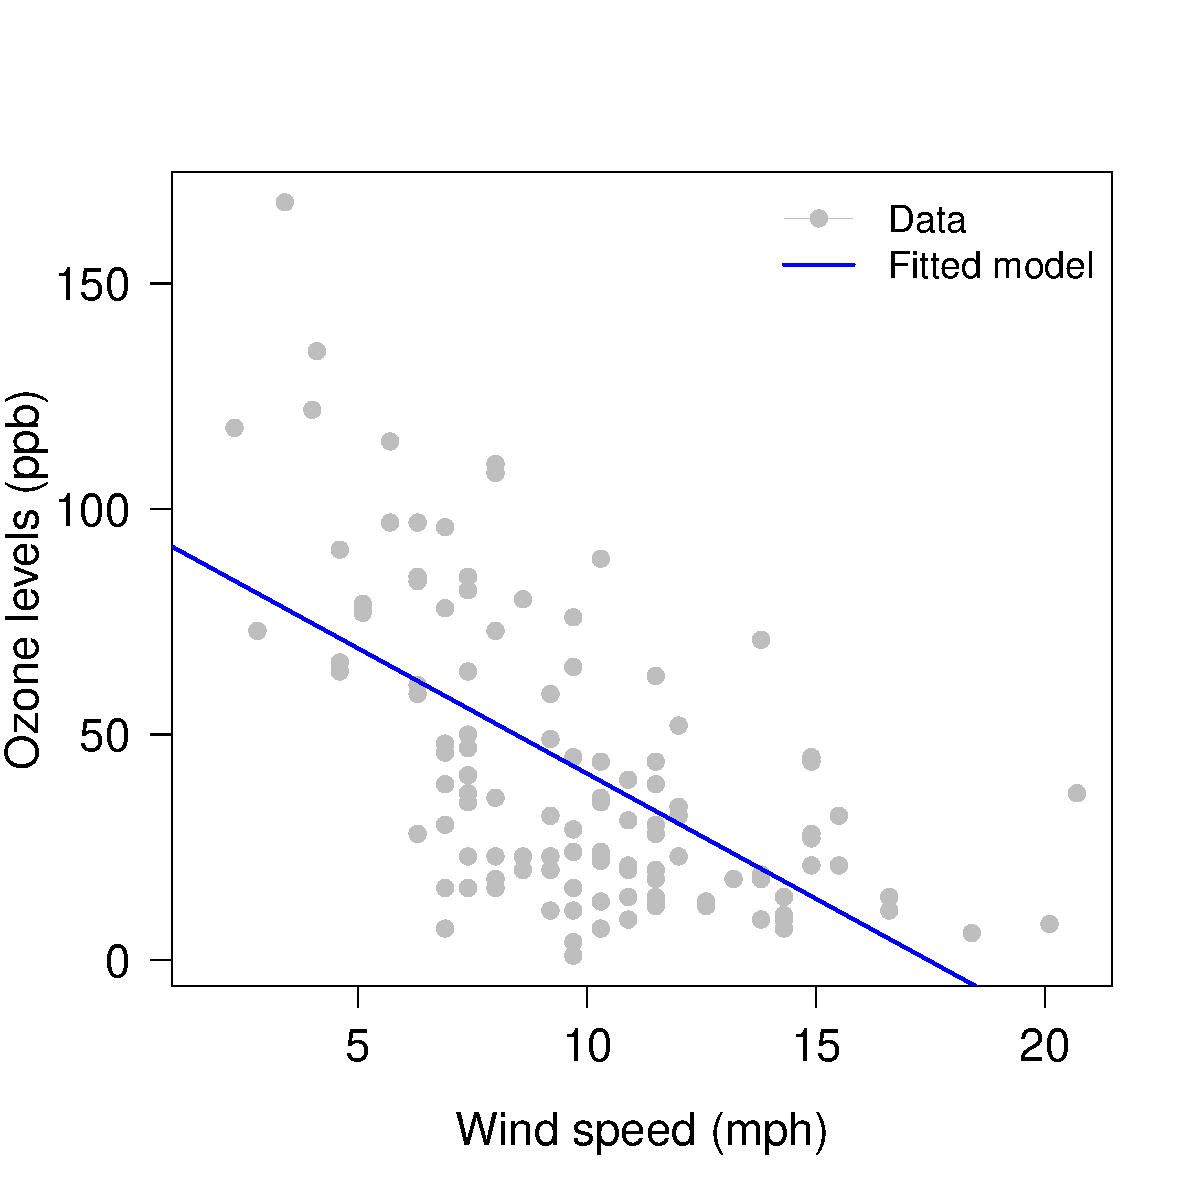
\includegraphics[width=0.45\textwidth]{figure/modelplot-1} 

}

\caption{\label{fig:modelplot}Scatter plot of ozone levels vs. wind speed and the fitted linear regression model for the mean of ozone levels as a function of wind speed. In the fitted model, \(\hat{\beta}_0 = 96.87\) ppb and \(\hat{\beta}_1 = -5.55\) ppb/mph.}\label{fig:modelplot}
\end{figure}

\end{knitrout}

%%%%%%%%%%%%%%%
%%%
%%% Section: Extracting
%%%
%%%%%%%%%%%%%%%
\section{Extracting \R\ code}
\label{sec:r}
You can extract the \R\ code included in the \Robject{Rnw} source document to a \R\ file by using the \Rfun{purl} function in the \Rpackage{knitr} package:

\begin{knitrout}\footnotesize
\definecolor{shadecolor}{rgb}{0.969, 0.969, 0.969}\color{fgcolor}\begin{kframe}
\begin{alltt}
\hldef{> }\hlkwd{library}\hldef{(knitr)}
\hldef{> }\hlkwd{purl}\hldef{(}\hlsng{"knitr_example.Rnw"}\hldef{)}
\end{alltt}
\end{kframe}
\end{knitrout}

Read \Rcode{?purl} to see how the \R\ code extraction can be customized (e.g., which chunks must be extracted, split \R\ files, file name or file documentation)


%%%%%%%%%%%%%%%
%%%
%%% References
%%%
%%%%%%%%%%%%%%%
\clearpage
\phantomsection %anchor
\bibliography{my_bibliography}







%%%%%%%%%%%%%%%
%%%
%%% Appendix
%%%
%%%%%%%%%%%%%%%
\clearpage


\appendix
\section{R code}
\label{app:Rcode}



\subsection{Libraries related to \Rpackage{knitr}}
\label{app:libraries}
\begin{knitrout}\footnotesize
\definecolor{shadecolor}{rgb}{0.969, 0.969, 0.969}\color{fgcolor}\begin{kframe}
\begin{alltt}
\hldef{> }\hlcom{### libraries related to knit:}
\hldef{> }\hlkwd{library}\hldef{(knitr)}
\hldef{> }\hlkwd{library}\hldef{(xtable)}     \hlcom{# to create nice LaTeX tables}
\end{alltt}
\end{kframe}
\end{knitrout}
  
  
\subsection{Plotting data}
\label{app:data}
\begin{knitrout}\footnotesize
\definecolor{shadecolor}{rgb}{0.969, 0.969, 0.969}\color{fgcolor}\begin{kframe}
\begin{alltt}
\hldef{> }\hlcom{### scatter plot ozone vs. wind:}
\hldef{> }\hlkwd{par}\hldef{(}\hlkwc{las} \hldef{=} \hlnum{1}\hldef{,} \hlkwc{cex.lab} \hldef{=} \hlnum{1.3}\hldef{,} \hlkwc{cex.axis} \hldef{=} \hlnum{1.3}\hldef{)}
\hldef{> }\hlkwd{plot}\hldef{(airquality}\hlopt{$}\hldef{Wind,}
\hldef{+ }     \hldef{airquality}\hlopt{$}\hldef{Ozone,}
\hldef{+ }     \hlkwc{xlab} \hldef{=} \hlsng{"Wind speed (mph)"}\hldef{,}
\hldef{+ }     \hlkwc{ylab} \hldef{=} \hlsng{"Ozone levels (ppb)"}\hldef{,}
\hldef{+ }     \hlkwc{pch} \hldef{=} \hlnum{19}\hldef{,}
\hldef{+ }     \hlkwc{col} \hldef{=} \hlsng{"gray"}\hldef{)}
\end{alltt}
\end{kframe}
\end{knitrout}
  
\subsection{Fitting the linear regression model}
\label{app:model}
\begin{knitrout}\footnotesize
\definecolor{shadecolor}{rgb}{0.969, 0.969, 0.969}\color{fgcolor}\begin{kframe}
\begin{alltt}
\hldef{> }\hlcom{### linear regression model fitting:}
\hldef{> }\hldef{mod} \hlkwb{<-} \hlkwd{lm}\hldef{(Ozone} \hlopt{~} \hldef{Wind,} \hlkwc{data} \hldef{= airquality)}
\hldef{> }\hlcom{### get coefficients table:}
\hldef{> }\hldef{coefs} \hlkwb{<-} \hlkwd{summary}\hldef{(mod)}\hlopt{$}\hldef{coefficients}
\hldef{> }\hlkwd{show}\hldef{(coefs)}
\hldef{> }\hlcom{### get beta of interest:}
\hldef{> }\hldef{beta} \hlkwb{<-} \hldef{coefs[}\hlsng{"Wind"}\hldef{,} \hlsng{"Estimate"}\hldef{]}
\end{alltt}
\end{kframe}
\end{knitrout}
  
  
\subsection{Plotting the fitted model}
\label{app:plotmodel}
\begin{knitrout}\footnotesize
\definecolor{shadecolor}{rgb}{0.969, 0.969, 0.969}\color{fgcolor}\begin{kframe}
\begin{alltt}
\hldef{> }\hlcom{# scatter plot ozone vs. wind again (recycling code in chunk dataplot):}
\hldef{> }
\hldef{> }\hlcom{# we increase the font sizes to compensate the reduction that dev='tikz'}
\hldef{> }\hlcom{# introduces: }
\hldef{> }\hlkwd{par}\hldef{(}\hlkwc{cex} \hldef{=} \hlnum{1.4}\hldef{)}
\hldef{> }
\hldef{> }\hlcom{# reuse the previous chunk named "dataplot":}
\hldef{> }
\hldef{> }\hlcom{### scatter plot ozone vs. wind:}
\hldef{> }\hlkwd{par}\hldef{(}\hlkwc{las} \hldef{=} \hlnum{1}\hldef{,} \hlkwc{cex.lab} \hldef{=} \hlnum{1.3}\hldef{,} \hlkwc{cex.axis} \hldef{=} \hlnum{1.3}\hldef{)}
\hldef{> }\hlkwd{plot}\hldef{(airquality}\hlopt{$}\hldef{Wind,}
\hldef{+ }     \hldef{airquality}\hlopt{$}\hldef{Ozone,}
\hldef{+ }     \hlkwc{xlab} \hldef{=} \hlsng{"Wind speed (mph)"}\hldef{,}
\hldef{+ }     \hlkwc{ylab} \hldef{=} \hlsng{"Ozone levels (ppb)"}\hldef{,}
\hldef{+ }     \hlkwc{pch} \hldef{=} \hlnum{19}\hldef{,}
\hldef{+ }     \hlkwc{col} \hldef{=} \hlsng{"gray"}\hldef{)}
\hldef{> }
\hldef{> }\hlcom{# add the fitted model line:}
\hldef{> }\hlkwd{abline}\hldef{(mod,} \hlkwc{col} \hldef{=} \hlsng{"blue"}\hldef{,} \hlkwc{lwd} \hldef{=} \hlnum{2}\hldef{)}
\hldef{> }
\hldef{> }\hlcom{# add legend:}
\hldef{> }\hlkwd{legend}\hldef{(}\hlsng{"topright"}\hldef{,}
\hldef{+ }       \hlkwc{legend} \hldef{=} \hlkwd{c}\hldef{(}\hlsng{"Data"}\hldef{,} \hlsng{"Fitted model"}\hldef{),}
\hldef{+ }       \hlkwc{col} \hldef{=} \hlkwd{c}\hldef{(}\hlsng{"gray"}\hldef{,} \hlsng{"blue"}\hldef{),}
\hldef{+ }       \hlkwc{lwd} \hldef{=} \hlkwd{c}\hldef{(}\hlnum{0}\hldef{,} \hlnum{2}\hldef{),}   \hlcom{# line width }
\hldef{+ }       \hlkwc{pch} \hldef{=} \hlkwd{c}\hldef{(}\hlnum{19}\hldef{,} \hlnum{NA}\hldef{),} \hlcom{# point symbol}
\hldef{+ }       \hlkwc{bty} \hldef{=} \hlsng{"n"}\hldef{,}       \hlcom{# no box around the legend}
\hldef{+ }       \hlkwc{cex} \hldef{=} \hlnum{1.1}\hldef{)}       \hlcom{# font size (multiplier)}
\end{alltt}
\end{kframe}
\end{knitrout}
  
  
\subsection{Exporting the table to \LaTeX}
\label{app:table}
\begin{knitrout}\footnotesize
\definecolor{shadecolor}{rgb}{0.969, 0.969, 0.969}\color{fgcolor}\begin{kframe}
\begin{alltt}
\hldef{> }\hlcom{# exporting coefficients table to LaTeX format:}
\hldef{> }\hldef{modtable} \hlkwb{<-} \hlkwd{xtable}\hldef{(coefs,}
\hldef{+ }                   \hlkwc{digits} \hldef{=} \hlkwd{c}\hldef{(}\hlnum{0}\hldef{,} \hlnum{2}\hldef{,} \hlnum{2}\hldef{,} \hlnum{2}\hldef{,} \hlnum{4}\hldef{),}
\hldef{+ }                   \hlkwc{caption} \hldef{=} \hlsng{"Linear regression model coefficients for wind and ozone association."}\hldef{,}
\hldef{+ }                   \hlkwc{label} \hldef{=} \hlsng{"tab:coeftable"}\hldef{)}
\hldef{> }\hlcom{# cosmetics for table head (LaTeX slash (\textbackslash{}) must be doubled inside a R chunk):}
\hldef{> }\hlkwd{colnames}\hldef{(modtable)} \hlkwb{<-} \hlkwd{c}\hldef{(}\hlsng{"\textbackslash{}\textbackslash{}multicolumn\{1\}\{c\}\{\textbackslash{}\textbackslash{}bf Estimate\}"}\hldef{,}
\hldef{+ }                        \hlsng{"\textbackslash{}\textbackslash{}multicolumn\{1\}\{c\}\{\textbackslash{}\textbackslash{}bf Std.~Error\}"}\hldef{,}
\hldef{+ }                        \hlsng{"\textbackslash{}\textbackslash{}multicolumn\{1\}\{c\}\{\textbackslash{}\textbackslash{}(\textbackslash{}\textbackslash{}boldsymbol\{t\}\textbackslash{}\textbackslash{})\textbackslash{}\textbackslash{}bf\{-value\}\}"}\hldef{,}
\hldef{+ }                        \hlsng{"\textbackslash{}\textbackslash{}multicolumn\{1\}\{c\}\{\textbackslash{}\textbackslash{}(\textbackslash{}\textbackslash{}boldsymbol\{p\}\textbackslash{}\textbackslash{})\textbackslash{}\textbackslash{}bf\{-value\}\}"}\hldef{)}
\hldef{> }
\hldef{> }\hlcom{# format and print the table:}
\hldef{> }\hlkwd{print}\hldef{(modtable,}
\hldef{+ }      \hlkwc{table.placement} \hldef{=} \hlsng{"ht"}\hldef{,}
\hldef{+ }      \hlkwc{size} \hldef{=} \hlsng{"footnotesize"}\hldef{,}
\hldef{+ }      \hlkwc{include.rownames} \hldef{=} \hlnum{TRUE}\hldef{,}
\hldef{+ }      \hlkwc{include.colnames} \hldef{=} \hlnum{TRUE}\hldef{,}
\hldef{+ }      \hlkwc{floating} \hldef{=} \hlnum{TRUE}\hldef{,}                 \hlcom{# whether \textbackslash{}begin\{table\} should be created (TRUE) or not (FALSE)}
\hldef{+ }      \hlkwc{sanitize.text.function} \hldef{= force,}  \hlcom{# important to treat content of columns as latex function}
\hldef{+ }      \hlkwc{booktabs} \hldef{=} \hlnum{TRUE}\hldef{)}                 \hlcom{# requires \textbackslash{}usepackage\{booktabs\} in the preamble of the document}
\end{alltt}
\end{kframe}
\end{knitrout}
  
\end{document}

